\documentclass[mgr, shortabstract]{iithesis}

\usepackage[utf8]{inputenc}
\usepackage{amsmath}
\usepackage{minted}
\usepackage{listings}
\usepackage{graphicx}

%%%%% DANE DO STRONY TYTUŁOWEJ
\polishtitle    {Polski tytuł}
\englishtitle   {English title}
%\polishabstract {\ldots}
%\englishabstract{\ldots}
\author         {Maksymilian Debeściak}
% w przypadku kilku promotorow, lub koniecznosci podania ich afiliacji, linie
% w ponizszym poleceniu mozna zlamac poleceniem \fmlinebreak
\advisor        {dr Jan Kowalski}
%\date          {}                     % Data zlozenia pracy

\polishabstract {Polskie streszczenie}
\englishabstract {Angielskie streszczenie}

% Dane do oswiadczenia o autorskim wykonaniu
%\transcriptnum {}                     % Numer indeksu
%\advisorgen    {dr. Jana Kowalskiego} % Nazwisko promotora w dopelniaczu
%%%%%

%%%%% WLASNE DODATKOWE PAKIETY
%
%\usepackage{graphicx,listings,amsmath,amssymb,amsthm,amsfonts,tikz}
%

%%%%% WŁASNE DEFINICJE I POLECENIA
%
%\theoremstyle{definition} \newtheorem{definition}{Definition}[chapter]
%\theoremstyle{remark} \newtheorem{remark}[definition]{Observation}
%\theoremstyle{plain} \newtheorem{theorem}[definition]{Theorem}
%\theoremstyle{plain} \newtheorem{lemma}[definition]{Lemma}
%\renewcommand \qedsymbol {\ensuremath{\square}}
% ...
%%%%%

\newmintedfile[swiftcode]{swift}{
  fontsize=\footnotesize
}

\newcommand{\todo}[1]{
  \textit{\textbf{TODO: }#1}
}

\newcommand{\ang}[1]{ang. \textit{#1}}

\begin{document}

%%%%% POCZĄTEK ZASADNICZEGO TEKSTU PRACY

\chapter{Wstęp}
\label{ch:wstep}

...

\chapter{Podobieństwa do innych języków programowania}
\label{ch:podobienstwa_do_innych}

\section{Podstawowe cechy}
\label{s:podstawowe_cechy}

Swift to wieloparadygmatowy język programowania łączący pomysły znane z innych popularnych języków, takich jak: Objective-C, C\#, Rust, Haskell czy Ruby. Podobnie jak C\#, pozwala na tworzenie struktur (value type/typów wartościowych?), klas (reference type/typów referencyjnych?) i typów wyliczeniowych. Wspiera również dziedziczenie (ale nie wielokrotne), definiowanie protokołów (odpowiednik interfejsów z C\# czy Java) oraz polimorfizm parametryczny (typy generyczne), nie pozwala natomiast na definiowanie klas abstrakcyjnych, zachęcając tym samym programistów do szerokiego stosowania interfejsów.

\todo{Tu przydałby się jeszcze jeden akapit o mniej znaczących feature'ach}

\section{Typy generyczne}
\label{s:typy_generyczne}

Swift wspiera dwie podstawowe koncepcje generyczności:
\begin{itemize}
  \item klasy, struktury, typy wyliczeniowe oraz funkcje z parametrami typu (ang. \textit{generics})
  \item protokoły z powiązanymi typami (ang. \textit{associated types})
\end{itemize}

Klasy (struktury, funkcje) ze zmiennymi typu to pomysł dobrze znany z większości popularnych języków pozwalających na programowania obiektowe, takich jak C\# czy Java. W momencie definiowania klasy programista ma możliwość zdefiniowania zmiennych przebiegających przestrzeń typów używanych w definiowanej klasie. Dodatkowo Swift oferuje kilka bardziej zaawansowanych mechnizmów związanych ze zmiennymi typu:

\todo{Ujednolicić nazewnictwo}
\begin{itemize}
  \item możliwość dodania ograniczeń na typy, po których przebiega zmienna, np. zmienna może być tylko typem implementującym dany protokół lub dziedziczącym po danej klasie
  \item automatyczna inferencja typów paremetrów generycznych
  \item możliwość nadawania aliasów funkcjom i typom generycznym
\end{itemize}
\todo{Coś o implementacji?}

W odróżnieniu od klas, struktur i funkcji, protokoły nie wspierają generycznych paremetrów typu. Zamiast tego, protokoły posiadają mechanizm typów powiązanych (\ang{associated types}), wzorowany na znanym np. ze Scali mechanizmie abstrakcyjnych pól typu (\ang{abstract type members}). Pozwala on na zdefiniowanie w protokole zmiennej typu, która zostanie ukonkretniona dopiero przez klasę implementującą dany protokół. Główną zaletą tego rozwiązania jest ukrycie typu podstawionego pod zmienną typu przed programistą używającym klasy implementującej dany protokół - typ podstawiony pod zmienną jest częścią implementacji i nie musi być jawnie podawany podczas tworzenie obiektu implementującego protokół.

\section{Typy wartościowe i referencyjne}

Podobnie jak w jęzuku C\#, typy w Swifcie można podzielić na dwie grupy:

\begin{itemize}
    \item typy wartościowe (\ang{value types})
    \item typy referencyjne (\ang{reference types})
\end{itemize}

Typy wartościowe to typy, które tworzą nowe instancje obiektów podczas przypisywania do zmiennej lub przekazywania do funkcji. Innymi słowy, każda instancja posiada swoją własną kopię danych, obiekty takie nie dzielą ze sobą stanu, przez co są łatwiejsze w zrozumieniu i bezpieczniejsze przy pracy z wieloma wątkami. Jeśli zmienna typu wartościowego zostanie zadeklarowana jako stała, cały obiekt, łącznie ze wszystkimi polami nie może zostać zmieniony. Typami wartościowymi w Swifcie są:

\begin{itemize}
    \item struktury
    \item typy wyliczeniowe
    \item krotki
\end{itemize}

Typy referencyjne to typy, których obiekty dzielą pomiędzy sobą te same dane, a podczas przypisywania lub przekazywania do funkcji tworzona jest tylko nowa referencja do tych samych danych. Zmienne typu referencyjnego zadeklarowane jako stałe zapewniają jedynie stałość referencji, jednak dane przypisane do zmiennej mogą być bez dowolnie zmieniane. Typami referencyjnymi w Swifcie są tylko klasy.

\section{Domknięcia jako typy pierwszoklasowe}

Podobnie jak w językach funkcyjnych i w większości nowoczesnych języków programowania obiektowego, domknięcia w Swifcie są typem pierwszoklasowym (\ang{first-class citizen}), tzn:

\begin{itemize}
    \item mogą być przechowywane w zmiennych i stanowić elementu struktur danych
    \item mogą być podawane jako parametry wywołania funkcji i metod
    \item mogą byc zwracane przez funkcje i metody
\end{itemize}

\section{Leniwość}

Swift jest domyślnie językiem z ewaluacją gorliwą, autorzy zaimplementowali jednak dwa rozwiązania pozwalające w podstawowym stopniu na wspieranie leniwych obliczeń. Po pierwsze, w Swifcie, podobnie jak w C\#, istnieje możliwość leniwej inicjalizacji obiektów. O ile jednak w C\# mechanizm ten polega na użyciu klasy $Lazy$ z biblioteki standardowej, o tyle w Swifcie jest on zaszyty w samym języku - służy do tego słowo kluczowe $lazy$.Drugim rozwiązaniem są leniwe struktury danych, których implementacja opera się na znanych również z języka C\# czy Java generatorach.

\section{Elementy zaczerpnięte z języków funkcyjnych}

Pomimo tego, że Swift był projektowany głównie jako język programowanie obiektowego, jego twórcy skupili dużą część swojej uwagi na elementach powiązanych z programowaniem funkcyjnym, które mogłyby pomóc programistom pisać bezpieczniejszy i bardziej czytelny kod obiektowy. Najważniejsze z nich to:

\begin{itemize}
    \item Typy wyliczeniowe z typami powiązanymi (\ang{associated types}), które wprowadzają do Swifta koncept podobny do konstruktorów typów z Haskella. Dzięki tym strukturom danych, programista może w funkcyjny deklarować nowe typy.

    \item Dzięki zwięzłej i eleganckiej składni oraz potraktowaniu domknięć na równi klasami i stukturami, Swift oferuje bardzo dobre wsparcie dla funkcji wyższego rzędu. Najbardziej jest to widoczne w implementacji kolekcji danych, które już w bibliotece standardowej posiadają najczęściej używane funkcje służące do manipulowania nimi, takie jak \texttt{filter}, \texttt{map}, \texttt{reduce} czy \texttt{flatMap}.

    \item Autorzy Swifta postawili bardzo duży nacisk na niemutowalność (\todo{lepsze słowo?}) danych, co przejawia się w całej składni języka, np. dostępne jest słowo odrębne słowo kluczowe \texttt{let} służące do deklarowania stałych, parametry przekazywane do funkcji są domyślnie stałymi, użycie typów wartościowych jest preferowane nad użyciem klas (również w bibliotece standardowej) itp.

    \item Swift posiada zaawansowany mechanizm \textit{pattern matchingu}, który można wykorzystać do dopasowywania typów wyliczeniowych, krotek i wyrażeń. Tak jak w wielu językach funkcyjnych, \textit{pattern matching} w Swifcie jest wyczerpujący (\ang{exhaustive}), co oznacza, że każda wartość, która może pojawić się podczas dopasowywania musi zostać obsłużona.

    \item Aby uniknąć problemów z wartością \texttt{nil}, w języku Swift każda zmienna musi zostać zainicializowana już w momencie deklaracji. Jeśli programista chce celowo stworzyć zmienną mogącą przyjmować \texttt{nil} jako wartość, powinien użyć typu \texttt{Optional<T>}, który w swojej konstrukcji jest bardzo podobny do monady \texttt{Maybe} znanej z Haskella. Istnieje nawet mechanizm zwany \textit{optional chaning}, który zachowuje się tak, jak operacja \texttt{>>=} dla monady \texttt{Maybe}.

\end{itemize}

\section{Zwięzłość składni}

Jednym z największych problemów podczas programowania w Objective-C była słaba czytelność kodu i bardzo rozwlekła składnia. Dlatego podczas projektowania Swifta jego autorzy bardzo mocno wzorowali się na językach bardzo zwięzłych i łatwych do czytania, takich jak Python czy Ruby. Zrezygnowano z plików nagłówkowych, wprowadzono dużo cukru syntaktycznego dla najcześciej stosowanych konstrukcji (jak np. operator \texttt{T?} dla typu \texttt{Optional<T>}), wprowadzono domyślną inferencję typów. Rysunek \ref{f:keynote} pokazuje różnice pomiędzy kodem napisanym w Objective-C, a takim samym kodem w Swift.

\begin{figure}[ht]
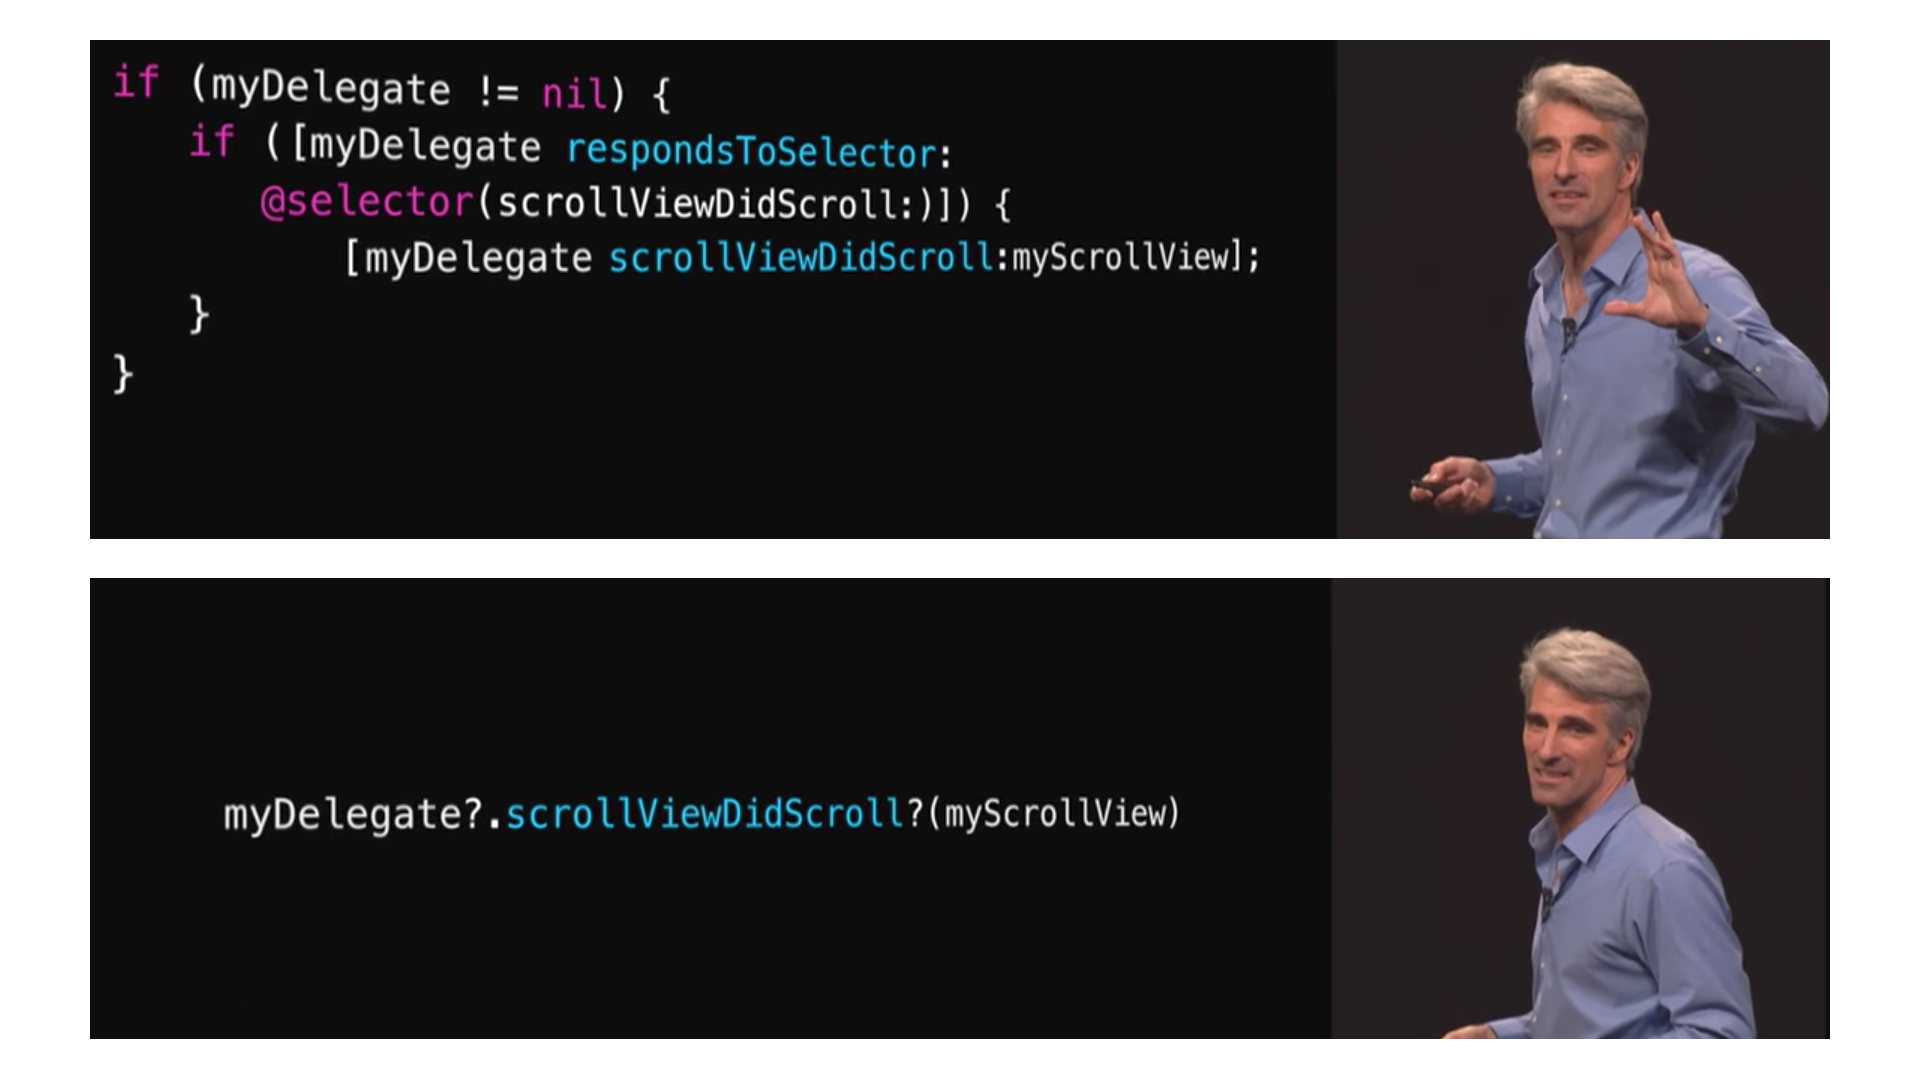
\includegraphics[width=0.99\textwidth]{images/Keynote.png}
\caption{Craig Federighi wskazuje różnice pomiędzy czytelnością kodu Objective-C (na górze) i Swift (na dole). \textit{WWDC Keynote 2014}}
\label{f:keynote}
\end{figure}

\section{Rozszerzenia typów}

Jedną z rzadziej spotykanych w językach statycznie typowanych językach programowania funkcjonalności jest możliwość rozszerzania istniejących już typów. Co prawda już w Objective-C programista miał moliwość stworzenia kategorii (\ang{category}), ale pozwalała ona tylko na dodawanie nowych funkcji, nie można było natomiast definiować nowych właściwości, konstruktorów ani typów zagnieżdżonych. Dlatego w Swifcie zotały zaimplementowane rozszerzenia (\ang{extensions}), które pozwalają na:

\begin{itemize}
    \item dodawanie nowych właściwości obliczanych (\ang{computed properties})
    \item definiowanie nowych metod instancji i metdo typu
    \item definiowanie nowych inicializatorów
    \item definiowanie i używanie typów zagnieżdżonych
    \item implementowanie metod protokołów
\end{itemize}

% Listingi

\newpage

\begin{listing}[ht]
  \swiftcode{src/2_1_class_struct_protocol_enum.swift}
  \caption{Przykładowe definicje podstwowych obiektów w Swift: struktury, klasy, protokołu i typu wyliczeniowego}
  \label{l:2_1_class_struct_protocol_enum}
\end{listing}

\begin{listing}[ht]
  \swiftcode{src/2_1_generics_and_inheritance.swift}
  \caption{Przykład klasy generycznej i klasy pochodnej w Swift}
  \label{l:2_1_generics_and_inheritance}
\end{listing}

\begin{listing}[ht]
  \swiftcode{src/2_1_associated_types.swift}
  \caption{Przykład protokołu z typem powiązanym w Swift}
  \label{l:2_1_associated_types}
\end{listing}

\begin{listing}[ht]
  \swiftcode{src/2_1_closures.swift}
  \caption{Przykład użycia domknięcia w Swift}
  \label{l:2_1_closures}
\end{listing}

\begin{listing}[ht]
  \swiftcode{src/2_1_laziness.swift}
  \caption{Przykład deklaracji leniwej zmiennej i leniwej sekwencji w Swift}
  \label{l:2_1_laziness}
\end{listing}

\begin{listing}[ht]
  \swiftcode{src/2_1_enum_with_associated_type.swift}
  \caption{Implementacja drzewa binarnego w Swift}
  \label{l:2_1_enum_with_associated_type}
\end{listing}

\begin{listing}[ht]
  \swiftcode{src/2_1_optional.swift}
  \caption{Typ \texttt{Optional} i mechanizm \textit{optional chaining}}
  \label{l:2_1_optional}
\end{listing}

%%%%% BIBLIOGRAFIA

%\begin{thebibliography}{1}
%\bibitem{example} \ldots
%\end{thebibliography}

\end{document}
